\chapter{Algorithms and Mathematics}
\label{ch:methodology}

\section{Overview}
\label{sec:method-overview}

This chapter states the model and the inference scheme in full. The model gives each flashcard
sequence one latent state on the logit scale. Between reviews the state moves as a mean-reverting
Ornstein--Uhlenbeck (OU) process, and at each review the recall outcome is a Bernoulli draw whose
probability is the logistic transform of the state. Parameters are shared through a hierarchy of
user and item effects, and the rate of forgetting may depend on the learner's earlier successes.
Inference uses a Gibbs-type sampler with P\'olya--Gamma augmentation, forward filtering backward
sampling (FFBS) for the latent path, and Metropolis--Hastings steps for the two parameters that
have no conjugate full conditional.

The notation follows the list of symbols. A card sequence is indexed by $n$. Each sequence is one
card of one user, and it contains reviews $t = 1, \dots, T_n$. The user of sequence $n$ is $u(n)$
and its item is $i(n)$, with $u = 1, \dots, U$ and $i = 1, \dots, I$. The total number of review events is $N$, and the number of transition terms with $t \ge 2$ is $N_{\mathrm{tr}}$. All latent states are scalars, so the model has dimension
$d = 1$. The recall outcome of review $t$ is $y_{n,t} \in \{0, 1\}$, where $y_{n,t} = 1$ when the
rating is greater than one. The grades Hard, Good and Easy are therefore treated as one class of
recall, a choice discussed as a limitation in Chapter~\ref{ch:conclusion}.

Figure~\ref{fig:tk_graphical_model} shows the dependence structure. Global parameters sit outside
the plates, user and item effects are drawn once per user or item, and the chain of latent states
is drawn once per sequence. The observed quantities are the outcomes $y_{n,t}$, the lagged outcomes
$X_{n,t}$ and the elapsed times $\Delta t_{n,t}$. The P\'olya--Gamma variables $\omega_{n,t}$ are
auxiliary, and they are introduced only to make the sampler tractable.

\begin{figure}[htbp]
  \centering
  % tk_graphical_model: directed graphical model with plates (DIAGRAMS.md item 22)
\begin{tikzpicture}[font=\footnotesize]
  % global parameters (outside every plate)
  \node[latent] (tb0) at (6.1,6.7) {$b_0$};
  \node[latent] (tg0) at (3.3,6.7) {$g_0$};
  \node[latent] (tla) at (7.5,6.7) {$\lambda$};
  \node[latent] (tka) at (9.0,6.7) {$\kappa$};
  \node[latent] (ts2) at (10.4,6.7) {$\sigma^2$};
  \node[latent] (tta) at (1.9,6.7) {$\tau^2_\alpha$};
  \node[latent] (ttb) at (0.4,6.7) {$\tau^2_\beta$};
  \node[latent] (ttg) at (4.7,6.7) {$\tau^2_\gamma$};
  % plates
  \draw[rounded corners=2pt, black!60] (0.2,2.4) rectangle (4.0,5.5);
  \node[anchor=south east, font=\footnotesize] at (3.9,2.5) {$u=1..U$};
  \draw[rounded corners=2pt, black!60] (0.2,0.2) rectangle (4.0,2.1);
  \node[anchor=south east, font=\footnotesize] at (3.9,0.3) {$i=1..I$};
  \draw[rounded corners=2pt, black!60] (4.6,0.2) rectangle (13.9,5.5);
  \node[anchor=north east, font=\footnotesize] at (13.8,5.4) {$n=1..N$};
  % user and item effects
  \node[latent] (al) at (1.2,3.6) {$\alpha_u$};
  \node[latent] (ga) at (2.9,3.6) {$\gamma_u$};
  \node[latent] (be) at (2.0,1.1) {$\beta_i$};
  % sequence n: chain psi_1 -> psi_2 -> ... -> psi_T, with mu, X, y, omega, Delta t
  \def\xa{5.9} \def\xb{8.3} \def\xT{12.1}
  \node[latent] (p1) at (\xa,2.6) {$\psi_{n,1}$};
  \node[latent] (p2) at (\xb,2.6) {$\psi_{n,2}$};
  \node[latent] (pT) at (\xT,2.6) {$\psi_{n,T}$};
  \node[obsnode] (y1) at (\xa,0.9) {$y_{n,1}$};
  \node[obsnode] (y2) at (\xb,0.9) {$y_{n,2}$};
  \node[obsnode] (yT) at (\xT,0.9) {$y_{n,T}$};
  \node[detnode] (m1) at (\xa,4.3) {$\mu_{n,1}$};
  \node[detnode] (m2) at (\xb,4.3) {$\mu_{n,2}$};
  \node[detnode] (mT) at (\xT,4.3) {$\mu_{n,T}$};
  \node[datasq] (x1) at (\xa+1.0,4.3) {$X_{n,1}$};
  \node[datasq] (x2) at (\xb+1.0,4.3) {$X_{n,2}$};
  \node[datasq] (xT) at (\xT+1.0,4.3) {$X_{n,T}$};
  \node[auxnode] (w1) at (\xa+0.9,1.7) {$\omega_{n,1}$};
  \node[auxnode] (w2) at (\xb+0.9,1.7) {$\omega_{n,2}$};
  \node[auxnode] (wT) at (\xT+0.9,1.7) {$\omega_{n,T}$};
  \node[datasq] (d2) at (\xb-1.2,3.5) {$\Delta t$};
  \node[datasq] (dT) at (\xT-1.2,3.5) {$\Delta t$};
  \node[font=\footnotesize] at (10.4,2.25) {$\cdots$};
  % arrows: chain, emissions, means, globals
  \draw[arrow] (p1) -- (p2);
  \draw[arrow] (p2) -- (pT);
  \draw[arrow] (p1) -- (y1); \draw[arrow] (p2) -- (y2); \draw[arrow] (pT) -- (yT);
  \draw[arrow] (m1) -- (p1); \draw[arrow] (m2) -- (p2); \draw[arrow] (mT) -- (pT);
  \draw[arrow] (x1) -- (m1); \draw[arrow] (x2) -- (m2); \draw[arrow] (xT) -- (mT);
  \draw[black!60] (w1) -- (p1); \draw[black!60] (w2) -- (p2); \draw[black!60] (wT) -- (pT);
  \draw[arrow] (d2) -- (p2); \draw[arrow] (dT) -- (pT);
  \draw[arrow] (tb0) -- (m1);
  \draw[arrow] (tla) to[bend right=10] (p1);
  \draw[arrow] (ts2) to[bend right=8] (p2);
  \draw[arrow] (tg0) -- (ga);
  \draw[arrow] (tta) -- (al);
  \draw[arrow] (ttb.south) -- (0.4,1.1) -- (be.west);
  \draw[arrow] (ttg) -- (ga);
  \draw[arrow] (al.north) to[out=90,in=180] (m1.west);
  \draw[arrow] (ga.east) -- (m1.west);
  \draw[arrow] (be.east) to[out=10,in=270] (m1.south);
  \draw[arrow] (tka) -- (tla);
\end{tikzpicture}

  \caption{Directed graphical model with plates. The plates are users ($u$), items ($i$) and card
    sequences ($n$). Shaded nodes are observed, dashed nodes are auxiliary P\'olya--Gamma variables,
    and squares are deterministic or data nodes. Global hyperparameters are outside the plates. The figure is a
    structural diagram and shows no fitted values.}
  \label{fig:tk_graphical_model}
\end{figure}

The remainder of the chapter follows the model from the inside out. Section~\ref{sec:method-ou}
gives the exact discretisation of the latent dynamics. Sections~\ref{sec:method-kappa} and
\ref{sec:method-mean} give the rate and the mean. Section~\ref{sec:method-observation} gives the
observation model. Sections~\ref{sec:method-pg} and \ref{sec:method-ffbs} give the two augmentation
and filtering steps. Section~\ref{sec:method-sweep} puts them into one sweep, and
Section~\ref{sec:method-prediction} describes how the fitted model predicts the next review.
Section~\ref{sec:method-diagnostics} states the convergence checks, and
Section~\ref{sec:method-why} discusses the choice of scheme and its costs.

\section{Ornstein--Uhlenbeck State Dynamics}
\label{sec:method-ou}

The latent state $\psi_{n,t}$ is the logit of the recall probability for sequence $n$ at review $t$.
Between reviews it follows an Ornstein--Uhlenbeck process,
\begin{equation}\label{eq:ou-sde}
  d\psi(s) = \lambda_{n,t}\,\bigl(\mu_{n,t} - \psi(s)\bigr)\,ds + \sigma\,dW(s),
\end{equation}
where $W$ is a standard Wiener process, $\sigma > 0$ is the diffusion scale, $\lambda_{n,t} > 0$ is
the rate at which the state is pulled back toward its equilibrium mean $\mu_{n,t}$ (Section
\ref{sec:method-mean}), and $\sigma^2$ is the diffusion variance. Over the gap that ends at review
$t$, the rate and the mean are held constant at their values for review $t$. The state therefore
drifts toward $\mu$ and is perturbed by noise, and recall probability falls when the state drifts
down.

The SDE has a closed-form solution over a gap, and this is what the model uses. Multiplying both
sides by the integrating factor $e^{\lambda_{n,t} s}$ and integrating over the gap
$\Delta t_{n,t}$ gives a linear recursion. The noise term is a Wiener integral with variance
given by the It\^o isometry,
\begin{equation}\label{eq:ou-var}
  \operatorname{Var}\!\bigl(w_{n,t}\bigr)
  = \sigma^2\int_0^{\Delta t_{n,t}} e^{-2\lambda_{n,t}(\Delta t_{n,t}-s)}\,ds
  = \sigma^2\,\frac{1-e^{-2\lambda_{n,t}\Delta t_{n,t}}}{2\lambda_{n,t}}.
\end{equation}
The exact transition from one review to the next is therefore
\begin{align}
  \psi_{n,t} &= \varphi_{n,t}\,\psi_{n,t-1} + (1-\varphi_{n,t})\,\mu_{n,t} + w_{n,t},
  \qquad w_{n,t} \sim \mathcal N(0,\, q_{n,t}), \label{eq:ou-recursion}\\
  \varphi_{n,t} &= e^{-\lambda_{n,t}\Delta t_{n,t}}, \label{eq:phi}\\
  q_{n,t} &= \sigma^2\,\frac{1-e^{-2\lambda_{n,t}\Delta t_{n,t}}}{2\lambda_{n,t}}. \label{eq:q}
\end{align}
Here $\varphi_{n,t}$ is the decay factor over the gap and $q_{n,t}$ is the transition variance. For
a $d$-dimensional linear SDE the same two quantities are computed with a matrix exponential, as in
the method of Van Loan \cite{vanloan1978computing}. For $d = 1$ the general step is not needed, since the closed forms above are exact. Given $\lambda$ and $\mu$ constant over each gap, this is an exact discretisation of the latent process, and no further approximation is introduced at this step. In code, $q$ is evaluated as $-\sigma^2\operatorname{expm1}(-2\lambda\Delta t)/(2\lambda)$,
which avoids cancellation when $\lambda\Delta t$ is small. The gap is clipped to
$\Delta t \in [0.01, 365]$ days before it enters Equations~\eqref{eq:phi} and \eqref{eq:q}.

The two limits explain the behaviour of the model. When $\lambda\Delta t \to 0$, we have
$\varphi \approx 1 - \lambda\Delta t$ and $q \approx \sigma^2\Delta t$, so the state behaves like a
random walk over short gaps. When $\lambda\Delta t \to \infty$, we have $\varphi \to 0$ and
$q \to \sigma^2/(2\lambda)$, so the state forgets its past and returns to the stationary variance.
Figure~\ref{fig:tk_ou_paths} shows the mean and the two-standard-deviation band for three rates,
and Figure~\ref{fig:tk_phi_q} shows $\varphi$ and $q$ as functions of the gap.

\begin{figure}[htbp]
  \centering
  % tk_ou_paths: OU mean and +-2 sd band (DIAGRAMS.md item 23); mu=2.3, m0=4, sigma^2=0.2
\begin{tikzpicture}
  \begin{axis}[width=13cm, height=7cm, xmin=0, xmax=30, ymin=-0.3, ymax=6,
    xlabel={$t$ (days)}, ylabel={$m(t)$ and $\pm 2\,\mathrm{sd}(t)$}, axis lines=left,
    legend pos=north east, legend style={font=\footnotesize, draw=none, fill=none},
    label style={font=\small}, tick label style={font=\footnotesize}]
    % lambda = 0.05: m = 2.3 + 1.7 e^{-0.05 t}; sd = sqrt(2 (1 - e^{-0.1 t}))
    \addplot[name path=u1, draw=none, forget plot, domain=0:30, samples=80] {2.3+1.7*exp(-0.05*x)+2*sqrt(2*(1-exp(-0.1*x)))};
    \addplot[name path=d1, draw=none, forget plot, domain=0:30, samples=80] {2.3+1.7*exp(-0.05*x)-2*sqrt(2*(1-exp(-0.1*x)))};
    \addplot[purple!14, forget plot] fill between[of=u1 and d1];
    % lambda = 0.4: sd = sqrt(0.25 (1 - e^{-0.8 t}))
    \addplot[name path=u2, draw=none, forget plot, domain=0:30, samples=80] {2.3+1.7*exp(-0.4*x)+2*sqrt(0.25*(1-exp(-0.8*x)))};
    \addplot[name path=d2, draw=none, forget plot, domain=0:30, samples=80] {2.3+1.7*exp(-0.4*x)-2*sqrt(0.25*(1-exp(-0.8*x)))};
    \addplot[teal!14, forget plot] fill between[of=u2 and d2];
    % lambda = 1.9: sd = sqrt((0.2/3.8)(1 - e^{-3.8 t}))
    \addplot[name path=u3, draw=none, forget plot, domain=0:30, samples=80] {2.3+1.7*exp(-1.9*x)+2*sqrt(0.2/3.8*(1-exp(-3.8*x)))};
    \addplot[name path=d3, draw=none, forget plot, domain=0:30, samples=80] {2.3+1.7*exp(-1.9*x)-2*sqrt(0.2/3.8*(1-exp(-3.8*x)))};
    \addplot[brown!16, forget plot] fill between[of=u3 and d3];
    % mean paths (drawn after the bands)
    \addplot[purple, thick, domain=0:30, samples=120] {2.3+1.7*exp(-0.05*x)};
    \addlegendentry{$\lambda=0.05$}
    \addplot[teal, thick, dashed, domain=0:30, samples=120] {2.3+1.7*exp(-0.4*x)};
    \addlegendentry{$\lambda=0.4$}
    \addplot[brown, very thick, dotted, domain=0:30, samples=120] {2.3+1.7*exp(-1.9*x)};
    \addlegendentry{$\lambda=1.9$}
  \end{axis}
\end{tikzpicture}

  \caption{Mean path and $\pm 2$ standard deviation band of the OU state for three rates
    ($\lambda = 0.05$, $0.4$ and $1.9$), started at $4$ with equilibrium mean $2.3$ and
    $\sigma^2 = 0.2$. These are illustrative values chosen for display, not fitted estimates. The
    band is $\pm 2$ times the standard deviation accumulated since time zero, so it widens and then
    levels off at the stationary value.}
  \label{fig:tk_ou_paths}
\end{figure}

\begin{figure}[htbp]
  \centering
  % tk_phi_q: phi and q against the gap (DIAGRAMS.md item 24); sigma^2 = 0.2
\begin{tikzpicture}
  \begin{groupplot}[group style={group size=2 by 1, horizontal sep=1.8cm},
    width=6.2cm, height=5.6cm, xmin=0, xmax=30, xlabel={$\Delta t$ (days)},
    label style={font=\small}, tick label style={font=\footnotesize}, title style={font=\small}]
    \nextgroupplot[ymin=0, ymax=1.05, ylabel={$\varphi(\Delta t)=e^{-\lambda\Delta t}$}, title={$\varphi$},
      legend pos=north east, legend style={font=\footnotesize, draw=none, fill=none}]
    \addplot[black, thick, domain=0:30, samples=120] {exp(-0.05*x)};
    \addlegendentry{$\lambda=0.05$}
    \addplot[black!70, thick, dashed, domain=0:30, samples=120] {exp(-0.4*x)};
    \addlegendentry{$\lambda=0.4$}
    \addplot[black!45, very thick, dotted, domain=0:30, samples=120] {exp(-1.9*x)};
    \addlegendentry{$\lambda=1.9$}
    \nextgroupplot[ymin=0, ymax=4.0, ylabel={$q(\Delta t)=\sigma^2(1-e^{-2\lambda\Delta t})/(2\lambda)$}, title={$q$},
      legend pos=north west, legend style={font=\footnotesize, draw=none, fill=none}]
    \addplot[black, thick, domain=0:30, samples=120] {0.2*(1-exp(-0.1*x))/0.1};
    \addlegendentry{$\lambda=0.05$}
    \addplot[black!70, thick, dashed, domain=0:30, samples=120] {0.2*(1-exp(-0.8*x))/0.8};
    \addlegendentry{$\lambda=0.4$}
    \addplot[black!45, very thick, dotted, domain=0:30, samples=120] {0.2*(1-exp(-3.8*x))/3.8};
    \addlegendentry{$\lambda=1.9$}
    % asymptotes sigma^2/(2 lambda), drawn last so they stay visible
    \addplot[black, densely dashed, domain=0:30] {2.0};
    \addplot[black!70, densely dashed, domain=0:30] {0.25};
    \addplot[black!45, densely dashed, domain=0:30] {0.0526316};
  \end{groupplot}
\end{tikzpicture}

  \caption{Decay factor $\varphi(\Delta t)$ (left) and transition variance $q(\Delta t)$ (right) for
    $\lambda = 0.05$, $0.4$ and $1.9$, with $\sigma^2 = 0.2$. The dashed lines in the right panel
    mark the stationary variance $\sigma^2/(2\lambda)$. The values are illustrative.}
  \label{fig:tk_phi_q}
\end{figure}

The first review of each sequence has no predecessor. For that review we set $\varphi_{n,1} = 0$
and $q_{n,1} = 1$, so the prior on the first state is $\psi_{n,1} \sim \mathcal N(\mu_{n,1}, 1)$.
This is the initialisation in the code, and it removes the need for an initial covariance $P_0$ in
the filter, because the first transition does not depend on $\psi_{n,0}$.

\section{Practice-Dependent Rate}
\label{sec:method-kappa}

The rate may depend on the learner's history through a single coefficient $\kappa$. Let $C_{n,t}$
be the logarithm of one plus the number of successful recalls before review $t$,
\begin{equation}\label{eq:C}
  C_{n,t} = \log\Bigl(1 + \sum_{s < t} y_{n,s}\Bigr),
\end{equation}
and define the rate as
\begin{equation}\label{eq:rate}
  \lambda_{n,t} = \lambda\,e^{-\kappa\,C_{n,t}},
\end{equation}
where $\lambda > 0$ is a base rate. The variant with $\kappa = 0$ uses a single constant rate and is
the learned-$\lambda$ model. The variant with $\kappa$ free is written $\text{Ours}+\kappa$ in the
results. When $\kappa > 0$, the rate falls as the number of successes grows, so the decay of the
state slows with practice. Figure~\ref{fig:tk_kappa_rate} shows the effective rate for three values
of $\kappa$.

\begin{figure}[htbp]
  \centering
  % tk_kappa_rate: effective rate against successful recalls (DIAGRAMS.md item 25); lambda = 1.5
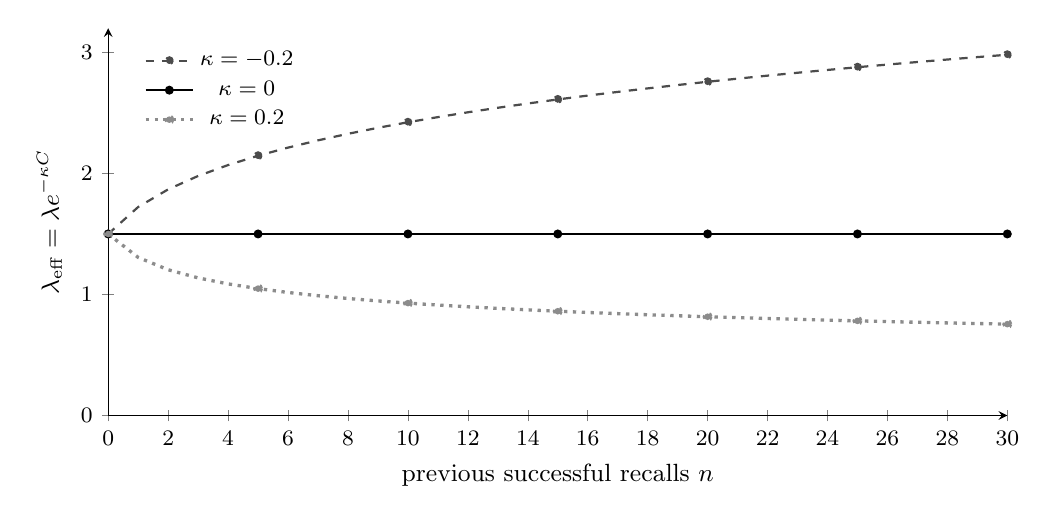
\begin{tikzpicture}
  \begin{axis}[width=13cm, height=6.5cm, xmin=0, xmax=30, ymin=0, ymax=3.2,
    xlabel={previous successful recalls $n$}, ylabel={$\lambda_{\mathrm{eff}}=\lambda e^{-\kappa C}$}, axis lines=left,
    legend pos=north west, legend style={font=\footnotesize, draw=none, fill=none},
    label style={font=\small}, tick label style={font=\footnotesize}]
    % C = log(1 + n); n = 0..30 (integer samples)
    \addplot[black!70, thick, dashed, mark=*, mark size=1.2pt, mark repeat=5, domain=0:30, samples=31] {1.5*exp(0.2*ln(1+x))};
    \addlegendentry{$\kappa=-0.2$}
    \addplot[black, thick, mark=*, mark size=1.2pt, mark repeat=5, domain=0:30, samples=31] {1.5*exp(0*ln(1+x))};
    \addlegendentry{$\kappa=0$}
    \addplot[black!45, very thick, dotted, mark=*, mark size=1.2pt, mark repeat=5, domain=0:30, samples=31] {1.5*exp(-0.2*ln(1+x))};
    \addlegendentry{$\kappa=0.2$}
  \end{axis}
\end{tikzpicture}

  \caption{Effective rate $\lambda_{\mathrm{eff}} = \lambda e^{-\kappa C}$ against the number of
    previous successful recalls $n$, with $C = \log(1+n)$, $\lambda = 1.5$ and
    $\kappa \in \{-0.2, 0, 0.2\}$. The values are illustrative. A positive $\kappa$ slows the decay
    as $n$ grows.}
  \label{fig:tk_kappa_rate}
\end{figure}

The coefficient $\kappa$ has the prior $\mathcal N(0,1)$ restricted to $|\kappa| < 3$, and it is
sampled only in the $\text{Ours}+\kappa$ variant. The sign of its estimate must be read with care.
In the benchmark run the fitted $\kappa$ is negative ($-0.160$), which would mean that decay speeds
up with practice, the opposite of the hypothesis that motivates $C_{n,t}$. Its chain did not
converge, as Chapter~\ref{ch:results} reports, so the value is not interpretable and this study does
not claim that practice slows decay. The variant with $\kappa$ is kept because it is part of the
model, and the comparison with the learned-$\lambda$ variant is reported as it is.

\section{Hierarchical Equilibrium Mean}
\label{sec:method-mean}

The equilibrium mean of the state is built from a global intercept, a user effect, an item effect
and a user-specific coefficient on the lagged outcome,
\begin{equation}\label{eq:mu}
  \mu_{n,t} = b_0 + \alpha_{u(n)} + \beta_{i(n)} + \gamma_{u(n)}\,X_{n,t},
  \qquad X_{n,t} = y_{n,t-1},\quad X_{n,1} = 0.
\end{equation}
Here $b_0$ is the global intercept, $\alpha_u$ is the effect of user $u$, $\beta_i$ is the effect of
item $i$ (the card-level effect in the list of symbols), and $\gamma_u$ is the slope on the lagged
outcome for user $u$. The lagged outcome $X_{n,t}$ is the recall outcome of the previous review of
the same sequence, and it is zero at the first review. It is not a practice count. A user with a
positive $\gamma_u$ therefore has a higher equilibrium mean after a recall than after a lapse, which
shifts the expected state at the next review.

The effects are partially pooled through a hierarchy,
\begin{equation}\label{eq:hier}
  \alpha_u \sim \mathcal N(0, \tau^2_\alpha), \qquad
  \beta_i \sim \mathcal N(0, \tau^2_\beta), \qquad
  \gamma_u \sim \mathcal N(g_0, \tau^2_\gamma),
\end{equation}
so each user's effects are shrunk toward the population values unless the data justify a larger
deviation. The population mean $g_0$ of the lagged-outcome slope is itself given a normal prior, and
each variance $\tau^2$ has an inverse-gamma hyperprior. Table~\ref{tab:priors} lists all priors.
The priors on $b_0$ and $g_0$ are wide, with variance 100. The variance parameters control the
amount of pooling, and their posterior is one of the quantities the diagnostics in
Section~\ref{sec:method-diagnostics} check.

\section{Observation Model}
\label{sec:method-observation}

The state is observed through a logistic link. Write
\begin{equation}\label{eq:logistic}
  \mathrm{logistic}(\psi) = \frac{1}{1+e^{-\psi}},
\end{equation}
so that the recall outcome of review $t$ satisfies
\begin{equation}\label{eq:obs}
  y_{n,t} \mid \psi_{n,t} \sim \mathrm{Bernoulli}\bigl(\mathrm{logistic}(\psi_{n,t})\bigr).
\end{equation}
The derivation notes write this function as $\sigma(\cdot)$. We use
$\mathrm{logistic}$ here because $\sigma$ already denotes the diffusion scale of the OU process.
The model has no separate observation-noise term. The binary outcome is a deterministic function of
$\psi$ up to the Bernoulli draw, and the uncertainty in the logit of recall is carried entirely by the
latent state.

\section{P\'olya--Gamma Augmentation}
\label{sec:method-pg}

The Bernoulli likelihood in $\psi$ is not Gaussian, so the FFBS step cannot be applied to it
directly. Polson, Scott and Windle \cite{polson2013pg} gave an identity that writes the logistic
likelihood as a Gaussian mixture in $\psi$. Let $k_{n,t} = y_{n,t} - \tfrac{1}{2}$. Then
\begin{equation}\label{eq:pg-identity}
  \frac{\bigl(e^{\psi_{n,t}}\bigr)^{y_{n,t}}}{1+e^{\psi_{n,t}}}
  = \frac{1}{2}\,e^{k_{n,t}\psi_{n,t}}
  \int_0^\infty e^{-\omega\psi_{n,t}^2/2}\,p_{\mathrm{PG}}(\omega \mid 1, 0)\,d\omega,
\end{equation}
where $p_{\mathrm{PG}}(\cdot \mid 1, 0)$ is the density of the P\'olya--Gamma distribution with
parameters $(1,0)$. We use $k_{n,t}$ rather than the symbol $\kappa$ to avoid a clash with the rate
coefficient of Section~\ref{sec:method-kappa}. Conditional on the auxiliary variable
$\omega_{n,t}$, the factor $e^{k\psi - \omega\psi^2/2}$ is proportional to a Gaussian kernel in
$\psi$. Completing the square gives a pseudo-observation,
\begin{equation}\label{eq:pseudo}
  z_{n,t} = \frac{k_{n,t}}{\omega_{n,t}}, \qquad \operatorname{Var}(z_{n,t}\mid \omega_{n,t}) = \frac{1}{\omega_{n,t}},
\end{equation}
so that, given $\omega$ and the parameters, the latent state is observed through a linear Gaussian
measurement. The auxiliary variable is drawn from its conditional,
$\omega_{n,t} \mid \psi_{n,t} \sim \mathrm{PG}(1, \psi_{n,t})$, which is the first step of the sweep.

The P\'olya--Gamma distribution has no closed-form sampler. The code draws $\omega$ from the infinite
series representation of Polson et al.,
\begin{equation}\label{eq:pg-series}
  \omega = \frac{1}{2\pi^2}\sum_{k=1}^{\infty}
  \frac{g_k}{(k-\tfrac{1}{2})^2 + c^2/(4\pi^2)},
  \qquad g_k \sim \mathrm{Gamma}(1,1),
\end{equation}
with $c = \psi_{n,t}$. The sum is truncated after $L = 200$ terms, so each draw is an approximation rather than an exact sample. Every term is positive, so dropping the tail biases each draw slightly low. The sampler is therefore an approximation to the scheme in Equation~\eqref{eq:pg-identity}. The conditional mean of the weight is
\begin{equation}\label{eq:pg-mean}
  \mathbb E[\omega \mid c] = \frac{\tanh(c/2)}{2c},
\end{equation}
which tends to $1/4$ as $c \to 0$. This mean is used in the one-step-ahead update of Section~\ref{sec:method-prediction}. Figure~\ref{fig:tk_pg_logistic} plots the link and this weight.

\begin{figure}[htbp]
  \centering
  % tk_pg_logistic: logistic and the Polya-Gamma mean weight (DIAGRAMS.md item 26)
\begin{tikzpicture}
  \begin{groupplot}[group style={group size=2 by 1, horizontal sep=1.6cm},
    width=6.2cm, height=5.4cm, xmin=-6, xmax=6, xlabel={$\psi$}, xtick={-6,-3,0,3,6},
    label style={font=\small}, tick label style={font=\footnotesize}, title style={font=\small}]
    \nextgroupplot[ymin=0, ymax=1.05, ylabel={$\mathrm{logistic}(\psi)$}, title={(a) observation model}]
    \addplot[black, thick, domain=-6:6, samples=121] {1/(1+exp(-x))};
    \nextgroupplot[ymin=0, ymax=0.3, ylabel={$E[\omega]=\tanh(\psi/2)/(2\psi)$},
      title={\shortstack{(b) PG(1, $\psi$) mean weight\\ = precision of pseudo-obs $z$}}]
    % tanh(psi/2) = (e^psi - 1)/(e^psi + 1); samples avoid psi = 0 exactly
    \addplot[black, thick, domain=-6:6, samples=120] {((exp(x)-1)/(exp(x)+1))/(2*x)};
    % marker last: the value 1/4 at psi = 0
    \addplot[only marks, mark=*, mark size=1.6pt, black] coordinates {(0,0.25)};
    \node[font=\footnotesize, anchor=east] at (axis cs:5.8,0.04) {$0.25$ at $\psi=0$};
  \end{groupplot}
\end{tikzpicture}

  \caption{Left: the logistic link $\mathrm{logistic}(\psi)$ of Equation~\eqref{eq:logistic}.
    Right: the conditional mean $\mathbb E[\omega \mid \psi] = \tanh(\psi/2)/(2\psi)$ of the
    P\'olya--Gamma weight, which equals $1/4$ at $\psi = 0$. This mean is the precision of the
    pseudo-observation $z$ in Equation~\eqref{eq:pseudo}, and it is used in the prediction step.}
  \label{fig:tk_pg_logistic}
\end{figure}

\section{Forward Filtering Backward Sampling}
\label{sec:method-ffbs}

Given the auxiliary variables $\omega$ and the parameters $\varphi$, $q$ and $\mu$, the latent
path of one sequence is a linear Gaussian state-space model. Its states are sampled jointly by
forward filtering backward sampling, as introduced for dynamic linear models by Carter and Kohn
\cite{carter1994gibbs} and by Fr\"uhwirth-Schnatter \cite{fruhwirth1994data}; see West and Harrison
\cite{west1997bayesian} for the general framework. The forward pass is a scalar Kalman filter. For
$t = 1, \dots, T$, the predicted mean and variance are
\begin{align}
  a_{n,t} &= \varphi_{n,t}\,m_{n,t-1} + (1-\varphi_{n,t})\,\mu_{n,t}, \label{eq:ffbs-a}\\
  R_{n,t} &= \varphi_{n,t}^2\,P_{n,t-1} + q_{n,t}, \label{eq:ffbs-R}
\end{align}
and the update with the pseudo-observation of Equation~\eqref{eq:pseudo} is
\begin{align}
  K_{n,t} &= \frac{R_{n,t}}{R_{n,t} + 1/\omega_{n,t}}, \label{eq:ffbs-K}\\
  m_{n,t} &= a_{n,t} + K_{n,t}\,(z_{n,t} - a_{n,t}), \qquad
  P_{n,t} = (1-K_{n,t})\,R_{n,t}. \label{eq:ffbs-m}
\end{align}
Because $\varphi_{n,1} = 0$, the initial values $m_{n,0}$ and $P_{n,0}$ do not affect the first
step. The backward pass draws the path from the last state to the first. The last state is drawn
from its filtered distribution, $\psi_{n,T} \sim \mathcal N(m_{n,T}, P_{n,T})$. For
$t = T-1, \dots, 1$, define
\begin{align}
  J_{n,t} &= \frac{P_{n,t}\,\varphi_{n,t+1}}{R_{n,t+1}}, \label{eq:ffbs-J}\\
  h_{n,t} &= m_{n,t} + J_{n,t}\,(\psi_{n,t+1} - a_{n,t+1}) \nonumber\\
  H_{n,t} &= P_{n,t} - J_{n,t}\,\varphi_{n,t+1}\,P_{n,t}, \label{eq:ffbs-H}
\end{align}
and draw $\psi_{n,t} \sim \mathcal N(h_{n,t}, H_{n,t})$. The draw is conditional on the later state
that was just sampled, so the whole path is a single draw from its joint conditional. Variances in
the code are floored at $10^{-12}$ to keep the Gaussian draws well defined. Per sequence, the cost is linear in its length. The kernel runs on a padded array, as described in Section~\ref{sec:method-complexity}. Figure~\ref{fig:tk_ffbs} shows the two passes schematically.

\begin{figure}[htbp]
  \centering
  % tk_ffbs: forward filter and backward sampling over psi (DIAGRAMS.md item 27)
\begin{tikzpicture}[font=\footnotesize]
  \foreach \i/\x in {1/1.2,2/3.9,3/6.6,4/9.3,5/12.0} {
    \node[latent] (s\i) at (\x,0) {$\psi_{\i}$};
    \node[datasq, align=center, minimum width=1.4cm, minimum height=0.9cm, font=\footnotesize] (z\i) at (\x,-3.4) {$z_\i$\\{\footnotesize var $1/\omega_\i$}};
    \draw[black!60, dotted] (s\i) -- (z\i);
  }
  % forward pass (Kalman filter), above the states
  \foreach \i in {1,2,3,4} {
    \pgfmathtruncatemacro{\u}{\i+1}
    \draw[darkblue, -{Stealth[length=2.4mm]}, thick] (s\i.north) to[bend left=40] (s\u.north);
  }
  \node[darkblue, font=\footnotesize, align=center] at (6.6,2.1) {forward: Kalman filter\\$a_t,\ R_t,\ m_t,\ P_t$};
  % backward pass (sampling), below the states
  \foreach \i in {4,3,2,1} {
    \pgfmathtruncatemacro{\u}{\i+1}
    \draw[green!50!black, -{Stealth[length=2.4mm]}, thick] (s\u.south) to[bend left=40] (s\i.south);
  }
  \node[green!50!black, font=\footnotesize, align=center, fill=white, inner sep=1pt] at (6.6,-1.45) {backward: sample $\psi_T \sim N(m_T, P_T)$,\\then $\psi_t \mid \psi_{t+1}$};
\end{tikzpicture}

  \caption{Forward and backward passes of FFBS for one sequence. The forward pass (blue) filters the
    states using the pseudo-observations $z_t$, whose variances are $1/\omega_t$. The backward pass
    (green) draws the last state from its filtered distribution and then each earlier state from its
    conditional given the next one. The diagram is schematic.}
  \label{fig:tk_ffbs}
\end{figure}

All sequences are processed in one compiled kernel. The implementation uses Numba
\cite{lam2015numba} with fast-math enabled, and it runs the forward and backward passes for every
sequence in a single call. 

\section{Metropolis-within-Gibbs Sweep}
\label{sec:method-sweep}

One iteration of the sampler, called a sweep, updates every block of unknowns in turn. Figure
\ref{fig:tk_gibbs_flow} shows the order, and Algorithm~\ref{alg:sweep} lists the steps. Most blocks
have conjugate full conditionals and are drawn directly. Two blocks, the log rate $\log\lambda$ and
the coefficient $\kappa$, do not, and they are updated by random-walk Metropolis--Hastings. The
sampler is therefore a Metropolis-within-Gibbs scheme, not a pure Gibbs sampler.

\begin{figure}[htbp]
  \centering
  % tk_gibbs_flow: one Gibbs sweep as a cycle (DIAGRAMS.md item 28)
\begin{tikzpicture}[font=\footnotesize]
  \tikzset{conj/.style={box, minimum width=2.7cm, minimum height=0.9cm, text width=2.5cm, font=\footnotesize},
    mh/.style={box, minimum width=2.7cm, minimum height=0.9cm, text width=2.5cm, font=\footnotesize,
      fill=orange!30, draw=orange!60!black}}
  % seven blocks on a circle (radius 4.2 cm), in sweep order
  \node[conj] (om) at (90:4.2)   {draw $\omega \mid \psi$ (PG)};
  \node[conj] (ps) at (38.6:4.2) {draw $\psi \mid \omega, \theta$ (FFBS)};
  \node[conj] (ef) at (-12.9:4.2) {draw $b_0, \alpha, \beta, \gamma, g_0$};
  \node[conj] (ta) at (-64.3:4.2) {draw $\tau^2_\alpha, \tau^2_\beta, \tau^2_\gamma$};
  \node[mh]   (la) at (-115.7:4.2) {MH on $\log\lambda$};
  \node[mh]   (ka) at (-167.1:4.2) {MH on $\kappa$ (optional)};
  \node[conj] (s2) at (141.4:4.2) {draw $\sigma^2$};
  % arrows, clockwise
  \draw[arrow] (om) -- (ps);
  \draw[arrow] (ps) -- (ef);
  \draw[arrow] (ef) -- (ta);
  \draw[arrow] (ta) -- (la);
  \draw[arrow] (la) -- (ka);
  \draw[arrow] (ka) -- (s2);
  \draw[arrow] (s2) -- (om);
  \node[font=\small, align=center] at (0,0) {one Gibbs sweep};
  % legend
  \node[box, fill=black!8, minimum width=0.6cm, minimum height=0.4cm, inner sep=0pt] (lg1) at (-4.6,-5.4) {};
  \node[anchor=west, font=\footnotesize] at (-4.3,-5.4) {conjugate draw};
  \node[box, fill=orange!30, draw=orange!60!black, minimum width=0.6cm, minimum height=0.4cm, inner sep=0pt] (lg2) at (-0.4,-5.4) {};
  \node[anchor=west, font=\footnotesize] at (-0.1,-5.4) {Metropolis--Hastings};
\end{tikzpicture}

  \caption{One Gibbs sweep as a cycle of seven blocks. Conjugate draws and Metropolis--Hastings
    (MH) updates are drawn differently, as the legend shows. The $\kappa$ block is present only in
    the $\text{Ours}+\kappa$ variant.}
  \label{fig:tk_gibbs_flow}
\end{figure}

\begin{algobox}{Metropolis-within-Gibbs sweep}\label{alg:sweep}
  Given the current state $(\psi, \omega, b_0, \alpha, \beta, \gamma, g_0, \tau^2, \lambda, \kappa, \sigma^2)$,
  one sweep performs the following steps in order.
  \begin{enumerate}[leftmargin=2em, itemsep=2pt]
    \item Draw $\omega_{n,t} \mid \psi \sim \mathrm{PG}(1, \psi_{n,t})$ for every event, truncated at $L = 200$ series terms.
    \item Draw the latent paths $\psi \mid \omega, \text{parameters}$ for all sequences by FFBS
      (Equations~\eqref{eq:ffbs-a}--\eqref{eq:ffbs-H}).
    \item Draw $b_0$, then $\alpha_u$, $\beta_i$, $\gamma_u$ and $g_0$, each from its conjugate
      Gaussian full conditional given $\psi$ (Section~\ref{sec:method-effects}).
    \item Draw each $\tau^2_\alpha$, $\tau^2_\beta$ and $\tau^2_\gamma$ from its inverse-gamma
      full conditional.
    \item Update $\log\lambda$ by random-walk Metropolis--Hastings, with five proposals per sweep and
      $\sigma^2$ integrated out of the target (Equation~\eqref{eq:lam-target}).
    \item If the $\kappa$ variant is used, update $\kappa$ by random-walk Metropolis--Hastings with
      five proposals per sweep.
    \item Draw $\sigma^2 \mid \psi, \lambda$ from its inverse-gamma full conditional
      (Equation~\eqref{eq:sigma2}).
  \end{enumerate}
  During burn-in, the proposal step sizes for $\lambda$ and $\kappa$ are adapted toward a
  $30\%$ acceptance rate (Section~\ref{sec:method-mh}). Only the kept draws are used after burn-in.
\end{algobox}

\subsection{Conjugate updates for the effects and the variances}
\label{sec:method-effects}

Given the latent path, the transition equation is a weighted linear regression in the effects. Write
the transition residual and its design as
\begin{equation}\label{eq:resid}
  r_{n,t} = \psi_{n,t} - \varphi_{n,t}\,\psi_{n,t-1}, \qquad d_{n,t} = 1 - \varphi_{n,t},
\end{equation}
so that
\begin{equation}\label{eq:resid-reg}
  r_{n,t} = d_{n,t}\,(b_0 + \alpha_{u(n)} + \beta_{i(n)} + \gamma_{u(n)} X_{n,t}) + w_{n,t},
  \qquad w_{n,t} \sim \mathcal N(0, q_{n,t}).
\end{equation}
For a group effect $\theta_g$ with prior $\mathcal N(m_0, v_0)$ and design value $x_{n,t}$, where $x_{n,t} = d_{n,t}$ for $b_0$, $\alpha$ and $\beta$, and $x_{n,t} = d_{n,t}X_{n,t}$ for $\gamma$, the full
conditional is normal with
\begin{equation}\label{eq:prec}
  \operatorname{prec}_g = \sum_{(n,t) \in g}\frac{x_{n,t}^2}{q_{n,t}} + \frac{1}{v_0},
  \qquad
  \operatorname{mean}_g = \operatorname{prec}_g^{-1}\Bigl(\sum_{(n,t) \in g}\frac{x_{n,t}\,r_{n,t}}{q_{n,t}} + \frac{m_0}{v_0}\Bigr).
\end{equation}
The sum runs over the reviews that belong to the group, and it includes first reviews. For a first review $\varphi = 0$ and $q = 1$, so $d = 1$ and $r_{n,1} = \psi_{n,1}$. The blocks are drawn one at a time, in the
order $b_0$, $\alpha$, $\beta$, $\gamma$ and then $g_0$, which is conjugate given $\gamma$. For the
prior $b_0 \sim \mathcal N(0, 100)$ we have $m_0 = 0$ and $v_0 = 100$.

Each variance hyperparameter has an inverse-gamma prior with shape $a_0 = 2$ and scale $b_\tau = 1$. Write
$\mathrm{IG}(a, b)$ for the density proportional to $x^{-a-1}e^{-b/x}$. If $G$ is the number of
groups in that effect, the full conditional of $\tau^2$ is
\begin{equation}\label{eq:tau}
  \tau^2_\bullet \mid \cdot \sim \mathrm{IG}\Bigl(a_0 + \frac{G}{2},\; b_\tau + \frac{1}{2}\sum_{g}(\theta_g - \text{centre}_g)^2\Bigr),
\end{equation}
where $\theta_g$ is the group effect and the centre is zero for $\alpha$ and $\beta$ and $g_0$ for
$\gamma$. The conditional for $\sigma^2$ is given in Section~\ref{sec:method-sigma}.

\subsection{Metropolis--Hastings updates for \texorpdfstring{$\lambda$}{lambda} and \texorpdfstring{$\kappa$}{kappa}}
\label{sec:method-mh}

The rate $\lambda$ enters the transition variance and the decay factor in a non-conjugate way, so
no standard full conditional is available. The sampler proposes on the log scale,
$\log\lambda' = \log\lambda + \epsilon$, with $\epsilon$ drawn from a normal distribution whose
standard deviation is the step size. The prior is $\log\lambda \sim \mathcal N(\log 0.05, 1.5^2)$,
restricted to $\lambda \in (10^{-4}, 20)$. The inverse-gamma noise scale $\sigma^2$ is integrated out
of the target. Define
\begin{align}\label{eq:S}
  e_{n,t} &= \psi_{n,t} - \varphi_{n,t}\psi_{n,t-1} - (1-\varphi_{n,t})\,\mu_{n,t},
  \\
  v_{n,t}(\lambda) &= \frac{1-e^{-2\lambda\Delta t_{n,t}}}{2\lambda}, \\
  Q(\lambda) &= \frac{1}{2}\sum_{n,\,t\ge 2}\frac{e_{n,t}^2}{v_{n,t}(\lambda)},\label{eq:Q}
\end{align}
where $\varphi$ depends on $\lambda$ through Equation~\eqref{eq:phi}, while $\mu$ does not depend on $\lambda$. The
log target is then
\begin{equation}\label{eq:lam-target}
  \log p(\lambda \mid \cdot) = -\frac{1}{2}\sum_{n,\,t\ge 2}\log v_{n,t}(\lambda)
  - \Bigl(a_\sigma + \frac{N_{\mathrm{tr}}}{2}\Bigr)\log\bigl(b_\sigma + Q(\lambda)\bigr)
  + \log p(\log\lambda) + \text{const},
\end{equation}
with $a_\sigma = 2$ and $b_\sigma = 0.5$ from the prior on $\sigma^2$. Here $N_{\mathrm{tr}}$ is the number of transition terms ($t \ge 2$) in the sums, and $N$ counts all review events. Five
proposals are made per sweep. The accepted value is used for the next state, and a rejected proposal
keeps the current value.

The coefficient $\kappa$ of the $\text{Ours}+\kappa$ variant is updated in the same way, with five
random-walk proposals per sweep under the prior $\mathcal N(0,1)$ restricted to $|\kappa| < 3$. Its target is the conditional posterior of $\kappa$ given the path, in which the rate of Equation~\eqref{eq:rate} enters the transition terms.

\subsection{Variance of the transition noise}
\label{sec:method-sigma}

Given the path and the rate, the diffusion variance has a conjugate update. With the prior
$\sigma^2 \sim \mathrm{IG}(a_\sigma, b_\sigma)$ and $Q$ as in Equation~\eqref{eq:Q} evaluated at the current $\lambda$,
\begin{equation}\label{eq:sigma2}
  \sigma^2 \mid \psi, \lambda \sim \mathrm{IG}\Bigl(a_\sigma + \frac{N_{\mathrm{tr}}}{2},\; b_\sigma + Q\Bigr).
\end{equation}
Both blocks use the same transition residuals, so they are coupled through $Q$. The Task 3 study in Chapter~\ref{ch:results} links the ridge between $\lambda$ and $\sigma^2$ to the ratio $\sigma^2/\lambda$.

\begin{table}[htbp]
  \centering
  \caption{Priors used by the sampler. The code defaults are shown. The inverse-gamma convention
    is shape $a$ and scale $b$, with density proportional to $x^{-a-1}e^{-b/x}$.}
  \label{tab:priors}
  \begin{tabular}{@{}>{\raggedright\arraybackslash}p{2.7cm}>{\raggedright\arraybackslash}p{5.4cm}>{\raggedright\arraybackslash}p{5.7cm}@{}}
    \toprule
    \textbf{Parameter} & \textbf{Prior} & \textbf{Notes}\\
    \midrule
    $\psi_{n,1}$ & $\mathcal N(\mu_{n,1}, 1)$ & First review: $\varphi = 0$ and $q = 1$\\
    $b_0$ & $\mathcal N(0, 100)$ & Global intercept\\
    $\alpha_u$ & $\mathcal N(0, \tau^2_\alpha)$ & User effect\\
    $\beta_i$ & $\mathcal N(0, \tau^2_\beta)$ & Item (card-level) effect\\
    $\gamma_u$ & $\mathcal N(g_0, \tau^2_\gamma)$ & User slope on the lagged outcome\\
    $g_0$ & $\mathcal N(0, 100)$ & Hyper-mean of $\gamma_u$\\
    $\tau^2_\alpha$, $\tau^2_\beta$, $\tau^2_\gamma$ & $\mathrm{IG}(2, 1)$ each & Hierarchical variances\\
    $\sigma^2$ & $\mathrm{IG}(2, 0.5)$ & OU diffusion variance\\
    $\log\lambda$ & $\mathcal N(\log 0.05, 1.5^2)$, $\lambda \in (10^{-4}, 20)$ & Base rate; random-walk MH\\
    $\kappa$ & $\mathcal N(0, 1)$, $\lvert\kappa\rvert < 3$ & Only in the $\text{Ours}+\kappa$ variant; random-walk MH\\
    \bottomrule
  \end{tabular}
\end{table}

\section{One-Step-Ahead Prediction}
\label{sec:method-prediction}

The model is evaluated by predicting each held-out review from the history before it. The parameters
are frozen at a set of posterior draws, and the latent state is filtered forward through the test
sequence. The evaluation protocol, including the leakage-free split, is defined in Chapter~\ref{ch:dataset}, and this section gives only the computation. For each of up to $S = 100$ draws, evenly spaced over the 250 kept draws, the procedure in Algorithm~\ref{alg:predict} runs one
filter. The prediction for review $t$ is then the average of the per-draw probabilities.

For a single draw, the predicted mean and variance of the state at review $t$ are given by the same
recursions as in the forward pass, Equations~\eqref{eq:ffbs-a} and \eqref{eq:ffbs-R}. The predictive
probability of recall integrates the logistic link over the Gaussian predictive distribution of the
state. We use the probit approximation to that integral,
\begin{equation}\label{eq:probit}
  p^{(g)}_{n,t} \approx \mathrm{logistic}\!\left(\frac{a_{n,t}}{\sqrt{1+\pi R_{n,t}/8}}\right),
\end{equation}
which is exact as the predictive variance tends to zero and is a common closed-form approximation to the logistic-normal integral. After the prediction is recorded, the filter is updated with the observed outcome $y_{n,t}$. The update uses the P\'olya--Gamma
mean at the predicted state as the weight,
\begin{equation}\label{eq:pred-update}
  \bar\omega_{n,t} = \frac{\tanh(a_{n,t}/2)}{2a_{n,t}}, \qquad
  z_{n,t} = \frac{y_{n,t} - \tfrac{1}{2}}{\bar\omega_{n,t}}, \qquad
  K_{n,t} = \frac{R_{n,t}}{R_{n,t} + 1/\bar\omega_{n,t}},
\end{equation}
followed by the same mean and variance update as Equation~\eqref{eq:ffbs-m}. The final prediction
averages the draws,
\begin{equation}\label{eq:pred-avg}
  \hat p_{n,t} = \frac{1}{S}\sum_{g=1}^{S} p^{(g)}_{n,t}.
\end{equation}

The update is an approximation. It replaces the P\'olya--Gamma variable by its conditional mean at the
predicted state, which is an assumed-density step, not the exact posterior update. It therefore does
not condition on $y_{n,t}$ in the way the full sampler does. The probit step is an approximation as
well. Together these mean that the predictions are approximate posterior predictive probabilities. Any log loss or calibration result therefore reflects the approximation as well as the model.

Algorithm~\ref{alg:predict} gives the steps as the code runs them. A warm card, one with at least one training review, starts from its last sampled training state $\psi_{\mathrm{last}}$ with variance $P = 0$. Its first test review uses $X$ equal to the last training outcome, and $C$ counts the training successes. Later test reviews use the outcomes of the reviews before them. A cold card, one with no training review, is handled differently. Its $\varphi = 0$ and $q = 1$ at every test review, so its latent state carries no memory from one test review to the next. Earlier test outcomes still enter the prediction through $X$ and $C$ in $\mu$ and $\lambda$. Cold cards account for 41,469 of the 95,400 scored events (43.5\%). This is an implementation limitation that uses less history than the protocol allows, not more, so it does not leak test labels. It is not corrected in the code, because that would change the reported run, and Chapters~\ref{ch:results} and \ref{ch:conclusion} report it.


\begin{algobox}{One-step-ahead prediction}\label{alg:predict}
  Input: $S \le 100$ posterior draws $g$ of $(b_0, \alpha, \beta, \gamma, \lambda, \kappa, \sigma^2)$
  evenly spaced over the kept draws; for each draw, the last sampled training state $\psi_{\mathrm{last}}$;
  the training and test sequences in time order.
  \begin{enumerate}[leftmargin=2em, itemsep=2pt]
    \item Freeze the parameters at draw $g$. Use zero effects for unseen users, items and cards
      (padding indices).
    \item For a warm card, start the filter at $\psi_{\mathrm{last}}$ with $P = 0$. For a cold card,
      set $\varphi = 0$ and $q = 1$ at every test review.
    \item For each test review $t$ in order, before its outcome is used, compute $a_{n,t}$ and $R_{n,t}$
      (Equations~\eqref{eq:ffbs-a} and \eqref{eq:ffbs-R}), with $X$ and $C$ taken from the history
      available so far.
    \item Record $p^{(g)}_{n,t} = \mathrm{logistic}\bigl(a_{n,t}/\sqrt{1+\pi R_{n,t}/8}\bigr)$.
    \item Update the filter with the observed $y_{n,t}$ (Equation~\eqref{eq:pred-update}). For a cold
      card this update has no effect on later reviews, because $\varphi = 0$ and $q = 1$.
    \item Repeat for every draw $g$, and set $\hat p_{n,t}$ to the average of the $S$ values
      (Equation~\eqref{eq:pred-avg}).
  \end{enumerate}
\end{algobox}

\section{Convergence Diagnostics}
\label{sec:method-diagnostics}

A sampler is useful only if its draws represent the posterior, and the diagnostics check this. The
standard check compares several chains started from different points. Write $\hat R$ for the split
potential scale reduction factor of Gelman and Rubin \cite{gelman1992inference}. Each chain is split
into halves, and with $M$ draws per half and $B$ and $W$ the between- and within-chain variances,
\begin{equation}\label{eq:rhat}
  \hat R = \sqrt{\frac{\frac{M-1}{M}\,W + \frac{1}{M}\,B}{W}}.
\end{equation}
Values near one indicate that the halves agree. The effective sample size (ESS) counts the draws
equivalent to independent ones, and it is reduced by autocorrelation at lags $\rho_k$,
\begin{equation}\label{eq:ess}
  \mathrm{ESS} = \frac{n}{1 + 2\sum_{m \ge 1}\Gamma_m},
\end{equation}
where $n$ is the number of draws, $\rho_k$ is the lag-$k$ autocorrelation, and $\Gamma_m = \rho_{2m-1} + \rho_{2m}$. The sum is cut at the first negative $\Gamma_m$ (Geyer's initial positive sequence), and the denominator is floored at one. The autocorrelations are computed with an FFT, as in the sampler's \texttt{ess} function. The Task 3 sampler study uses the rank-normalised form
of $\hat R$ and separate bulk and tail ESS, as recommended by Vehtari et al. \cite{vehtari2021rank}.
Its gate requires $\hat R < 1.01$ and an ESS of at least 400 for every monitored scalar.

The benchmark run is weaker than this. It used one chain with a fixed seed, so only the split
$\hat R$ and the ESS of the 250 kept draws are available. The chain did not converge. The rate
$\lambda$ had a split $\hat R$ of 2.44 and an ESS of 3.0, and several other scalars were also above
1.01 or had very small ESS. The full table is in Chapter~\ref{ch:results}. Because of this, the
benchmark scores of the proposed model are provisional. An 8000-iteration rerun was started to
address this, but it was stopped at sweep 1400 of 8000 before it finished. Its state was still
drifting, and it has no result, so the convergence question is open.

\section{Why This Inference Scheme}
\label{sec:method-why}

The scheme was chosen because it gives posterior draws of the latent path and of the parameters
within a single framework, and because most of its steps have closed forms. Its benefits and its
costs are both real, and this section states both.

The benefits are these. Polson et al. \cite{polson2013pg} make the logistic likelihood Gaussian given
the auxiliary variables, so the latent path can be drawn exactly by FFBS in each sweep. Most blocks
(the effects, the variance hyperparameters and the diffusion variance) have conjugate updates, so the
code does not need gradients, learning rates or other optimiser settings for them. The posterior draws
give a spread for each parameter and each latent state, and the prediction averages over the draws
rather than using a single fitted value. A point estimator such as HLR \cite{settles2016trainable} returns one fitted value per parameter. The sampler instead returns a set of draws, which is the main reason for the Bayesian treatment in this report, although whether the spread improves predictions is an empirical question. The design also builds on a well-established line of state-space
work \cite{carter1994gibbs,fruhwirth1994data,west1997bayesian}.

The costs are equally real. The sampler is slow. The benchmark fit took 27,530 seconds, about 7.6
hours on one core, and the prediction step took 1,266 seconds. The non-conjugate blocks need
Metropolis--Hastings steps with a step size adapted during burn-in, so their behaviour depends on
tuning as well as on the data. The mixing is poor for two structural reasons. When $\lambda\Delta t$
is large the transition variance depends mainly on the ratio $\sigma^2/\lambda$, which the Task 3 study links to a ridge between $\lambda$ and $\sigma^2$. When $\lambda\Delta t$ is small the
transition carries little information about $\lambda$. In addition, the mean design matrix has more
columns than its rank, so some combinations of the intercept and the effects are not identified by
the likelihood. The Task 3 study in Chapter~\ref{ch:results} found that no full-model fit passed the
convergence gate on the synthetic or real datasets it used, so the sampler as configured has not been shown to be reliable for the full model. The approximations in the P\'olya--Gamma truncation and in the prediction step
add a bias that this study has not measured.

Several alternatives exist, and none was tested in this report. Variational inference is generally
faster, and it turns posterior estimation into optimisation, but mean-field approximations often
understate posterior spread, and that would weaken the uncertainty argument above. A sampler that
updates the full path and every parameter by plain Metropolis--Hastings would need no augmentation,
but a random walk over a high-dimensional state with many effects would need careful proposal tuning,
and its mixing was not measured here. Integrated nested Laplace approximation is designed for latent
Gaussian models, and the logistic observation is not Gaussian, so it would need an extra
approximation. Neural sequence models can represent more flexible dependence on history, but they typically need more data than this model, and their parameters are harder to interpret.
Interweaving \cite{yu2011interweaving} is a known remedy for the centring problems described above.
It is only a pilot in this work, with no results, and it is discussed as future work in
Chapter~\ref{ch:conclusion}. The choice of scheme is therefore a trade-off, and this study does not
show that another scheme would be better or worse on the same data.

\section{Complexity}
\label{sec:method-complexity}

Table~\ref{tab:complexity} gives the cost of each step of one sweep. The FFBS kernel works on a padded array with $N_{\mathrm{seq}}$ rows and $T_{\max}$ columns, so its cost and memory are $O(N_{\mathrm{seq}}\,T_{\max})$. This is about $O(N)$ when sequence lengths are similar, and it is larger when a few sequences are long and padding dominates. The P\'olya--Gamma step costs $O(NL)$ with $L = 200$ terms. The prediction step costs $O(S\,N_{\mathrm{test}})$ over the $S \le 100$ draws and the held-out events, and it does not depend on the sweep count.

\begin{table}[htbp]
  \centering
  \footnotesize\setlength{\tabcolsep}{4pt}
  \caption{Cost of one Metropolis-within-Gibbs sweep, by step. $N$ is the number of review events,
    $N_{\mathrm{tr}}$ the transition terms ($t \ge 2$), $N_{\mathrm{seq}}$ the number of sequences,
    $T_{\max}$ the longest sequence, $L = 200$ the P\'olya--Gamma series terms, and $U$ and $I$ the
    numbers of users and items.}
  \label{tab:complexity}
  \begin{tabular}{@{}>{\raggedright\arraybackslash}p{5.0cm}>{\raggedright\arraybackslash}p{3.4cm}>{\raggedright\arraybackslash}p{5.6cm}@{}}
    \toprule
    \textbf{Step} & \textbf{Cost per sweep} & \textbf{Remarks}\\
    \midrule
    1. P\'olya--Gamma draws & $O(NL)$ & Truncated series with $L = 200$ terms\\
    2. FFBS (latent paths) & $O(N_{\mathrm{seq}}\,T_{\max})$ & Padded array; about $O(N)$ for similar lengths\\
    3. Effects $b_0$, $\alpha$, $\beta$, $\gamma$, $g_0$ & $O(N + U + I)$ & Sums over reviews, including first reviews\\
    4. Hierarchical variances $\tau^2$ & $O(U + I)$ & Inverse-gamma draws over groups\\
    5. Rate $\lambda$ (MH, 5 proposals) & $O(5N_{\mathrm{tr}})$ & Each proposal re-evaluates the transition terms\\
    6. Coefficient $\kappa$ (MH, 5 proposals) & $O(5N_{\mathrm{tr}})$ & Only in the $\text{Ours}+\kappa$ variant\\
    7. Diffusion variance $\sigma^2$ & $O(N_{\mathrm{tr}})$ & Inverse-gamma draw from $Q(\lambda)$\\
    \midrule
    Memory (all steps) & $O(N_{\mathrm{seq}}\,T_{\max})$ & Paths, auxiliary variables and residuals\\
    Prediction (outside the sweep) & $O(S\,N_{\mathrm{test}})$ & $S \le 100$ draws, held-out events\\
    \bottomrule
  \end{tabular}
\end{table}

At the scale of the benchmark, which has 100 users and at most 1000 cards per user, the sweep takes about 14 seconds (27,530 s / 2,000 $\approx$ 13.8 s in the benchmark fit), so the 2000 iterations of one chain dominate the cost of the reported run. The prediction step and the FSRS baselines take far less time, and the timings are reported in
Chapter~\ref{ch:results}.

\section{Improved Models: v2, v3 and GBDT}
\label{sec:method-improved}

The model of the previous sections is the proposed Bayesian model, and Experiments 2 and 3 evaluate it
(Chapter~\ref{ch:results}). After those experiments three further models were built to ask how much of
the remaining error is due to the memory model and how much to the learner and the data. They are
reported in Experiment 4. Two of them are cheaper variants of the Bayesian idea (v2 and v3), and the
third is a gradient-boosted tree model with no memory equation at all (GBDT). The proposed model
remains the one the title of this report refers to. This section states what v2, v3 and the GBDT
compute. It does not claim that they are better in general; Chapter~\ref{ch:results} gives the
evidence and the caveats.

\subsection{Model v2: hierarchical FSRS-style, fitted by MAP}
\label{sec:method-v2}

Model v2 (module \texttt{ours\_v2}) keeps the functional forms of FSRS-6 for the memory state of a card:
a stability $S$, a difficulty $D$, and a power-law forgetting curve $R(t, S) = (1 + F\,t/S)^{-d}$ with
decay $d$ and a constant $F$ fixed by $d$. The stability update after a recall, the update after a
lapse, the same-day update and the difficulty update have the FSRS-6 form. The $21$ global weights
$\mathbf{w}$ of these forms start at the FSRS-6 defaults, but unlike the default FSRS-6 baseline they are
learned jointly from all users of the training data. What is added is a hierarchy over users. Each user
$u$ has a vector of six random effects $\mathbf{e}_u$ that shift the initial stability, the growth after a
recall, the decay, the stability after a lapse, a logit bias on the predicted recall, and the initial difficulty. The effects are
non-centred,
\begin{equation}
  \mathbf{e}_u = \boldsymbol{\tau} \odot \mathbf{z}_u, \qquad \mathbf{z}_u \sim \mathcal{N}(\mathbf{0}, \mathbf{I}),
  \label{eq:v2-effects}
\end{equation}
with one learned global scale in $\boldsymbol{\tau}$ for each effect. A user with few reviews stays close
to the pooled model, and a user with many reviews can move away from it (partial pooling). The predicted
recall probability of a review is $R(t, S_u)$ computed from the replay of the card's earlier reviews with the
user's shifted weights, and the logit bias is added on the logit scale.

The decisive difference from the proposed Bayesian model is the inference. Model v2 maximises the posterior
over $\mathbf{w}$, $\boldsymbol{\tau}$ and the $\mathbf{z}_u$ by gradient ascent in PyTorch (maximum a posteriori, MAP).
It returns point estimates and no posterior samples, so it has no credible intervals and no convergence
diagnostics of the kind in Section~\ref{sec:method-diagnostics}. It is a hierarchical model in structure
and not a Bayesian one in inference. The frozen setting is $20$ epochs. The card replay is vectorised over
all cards, so a fit takes seconds on the Anki benchmark and minutes on Duolingo, instead of hours for MCMC.

\subsection{Model v3: v2 with a penalty, a lag term and a card effect}
\label{sec:method-v3}

Model v3 (module \texttt{ours\_v3}) adds three components to v2. First, a penalty on the squared scales
$\boldsymbol{\tau}$ of the user effects, with weight $300$ (the \texttt{tau\_pen} setting). The scales are positive through a softplus of a free parameter, and the objective is divided by the number of scored reviews of the fit set,
\begin{equation}
  \mathcal{L}_{\mathrm{v3}} = \mathcal{L}_{\mathrm{v2}} + \tfrac{1}{2}\,\lambda_{\tau}\,\lVert \boldsymbol{\tau} \rVert_2^2,
  \qquad \lambda_{\tau} = 300,
  \label{eq:v3-penalty}
\end{equation}
where $\mathcal{L}_{\mathrm{v2}}$ is the negative log posterior of v2. This penalty was the component that
mattered in the experiments, because it keeps the user effects from overfitting. Second, a lagged-outcome
term adds $b_{\mathrm{lag}}\,(2 y_{\mathrm{prev}} - 1)$ to the logit, where $y_{\mathrm{prev}}$ is the outcome of the card's
previous review and $b_{\mathrm{lag}}$ is one global weight. Third, a per-card logit effect with a fixed scale of $0.2$
(\texttt{card\_tau}). The card effect was not separately supported by the data: removing it changed the
validation log loss by less than $0.0001$. Model v3 is still fitted by MAP.

\subsection{GBDT: gradient-boosted trees without a memory equation}
\label{sec:method-gbdt}

The GBDT (module \texttt{gbdt}) is a LightGBM model \cite{ke2017lightgbm}, a gradient-boosted
decision tree ensemble \cite{friedman2001greedy}. It has no latent state, no forgetting curve and no
stability. It maps a feature vector of each review to a recall probability with a logistic loss. All
features use only information that precedes the review, as Table~\ref{tab:gbdt-features} lists.

\begin{table}[htbp]
  \centering
  \caption{Feature groups of the GBDT. Every feature is computed from reviews that precede the scored review,
    and the lexeme rate is available on Duolingo only.}
  \label{tab:gbdt-features}
  \begin{tabular}{@{}>{\raggedright\arraybackslash}p{3.4cm}>{\raggedright\arraybackslash}p{6.2cm}>{\raggedright\arraybackslash}p{4.2cm}@{}}
    \toprule
    \textbf{Group} & \textbf{Features} & \textbf{Note}\\
    \midrule
    Gap & Elapsed time since the card's previous review; its logarithm; a same-day indicator; the raw elapsed time in days from the logs (\texttt{dt\_days}) & Time since the last review of the card\\
    Card history & Review count, number of lapses, running recall rate; the last three grades, outcomes and gaps; time since the first review & Past reviews of this card\\
    FSRS-6 state & Stability $S$, difficulty $D$ and retrievability $R$ of the default FSRS-6 replayed over the card's history; their derived logit and ratio terms & Default weights, not fitted\\
    Running user statistics & Recall rate and review counts of the user so far, recent recall, reviews today and time since the user's last review & Cross-card ability signal\\
    Lexeme rate & Smoothed recall rate of the item over other training rows (smoothing constant $3$) & Duolingo only\\
    \bottomrule
  \end{tabular}
\end{table}

The frozen configuration has $15$ leaves per tree, a learning rate of $0.02$, and the smoothing constant $3$.
The model is trained on all non-first reviews of the training data, and the number of boosting rounds is
set by early stopping on a holdout taken from the fit data (the best iteration on Anki was $975$). The
configuration was chosen on validation data only: the last $20\%$ of each user's training days. The rule,
fixed before the runs, was the lowest mean validation log loss over both datasets among the variants that were not
significantly worse than FSRS-6 (optimised) on either dataset. Six stacked combinations were tried, and none
beat the GBDT alone, so the GBDT alone is the final model.

\paragraph{Leakage rules.}
A tree model with many history features can leak the answer easily, so the features follow four rules.
(i) A feature of a review uses only reviews that are earlier in time. (ii) The features of train rows
that need an aggregate over other rows, namely the smoothed lexeme rate, are computed out of fold.
(iii) Rows with the same timestamp are grouped: Duolingo records one practice session at a single
timestamp, so reviews in the same session must not see each other's outcomes. A first version of the GBDT
did not group them and leaked, which Chapter~\ref{ch:results} reports. (iv) The split and the scored rows are those
of Chapter~\ref{ch:dataset}, unchanged. The GBDT does not use the history counters supplied with the Duolingo logs or the
state column of the Anki logs.

\paragraph{Related approaches.}
Models of this type are not new in this field. DASH \cite{lindsey2014improving} and
DAS3H \cite{choffin2019das3h} are logistic models of past practice, KARL \cite{shu2024karl} uses
knowledge-aware retrieval and representations, and the winning submission of the Second Language
Acquisition Modeling task \cite{settles2018slam} was an ensemble of LightGBM and a recurrent
network \cite{osika2018slam}. The open benchmark \texttt{srs-benchmark} \cite{srsbenchmark} compares
spaced-repetition models on about ten thousand Anki users. What is specific to this report is the combination of tree
models with FSRS-state features, a leakage-audited protocol on two datasets, and the comparison
with a Bayesian model.

\subsection{What the three models are for}
\label{sec:method-improved-purpose}

The GBDT is a pure predictor: it has no stability or difficulty state, so it cannot by itself drive a
scheduler. The Bayesian models and v2 and v3 keep an interpretable memory state. Experiment~4 therefore
compares models of two kinds, and Chapter~\ref{ch:conclusion} discusses the trade-off.

\section{Summary}
\label{sec:method-summary}

The model places one latent logit state per card sequence on the Ornstein--Uhlenbeck transition
with decay $\varphi = e^{-\lambda\Delta t}$ and variance $q$ given by Equations~\eqref{eq:phi} and
\eqref{eq:q}. Its equilibrium mean is a hierarchical sum of a global intercept, user and item effects,
and a user slope on the lagged outcome. The rate may be scaled by a practice coefficient $\kappa$. Each
recall outcome is a Bernoulli draw through the logistic link. The sampler introduces
P\'olya--Gamma variables, draws the latent paths by FFBS, and updates the effects and variances
conjugately. The rate $\lambda$ and, in one variant, the coefficient $\kappa$ are updated by
Metropolis--Hastings. Prediction averages per-draw probit approximations after an approximate
P\'olya--Gamma update. The approximations, the truncated series and the single unconverged chain are
the main limitations of this chapter's scheme, and they are the basis for the caveats in
Chapter~\ref{ch:results}. Section~\ref{sec:method-improved} adds three later models, two MAP variants of the hierarchy (v2, v3) and a gradient-boosted tree model (GBDT) with no memory equation, which Experiment~4 evaluates. Chapter~\ref{ch:implementation} describes how the code implements these steps.
